\documentclass[aspectratio=43]{beamer}
% Theme works only with a 4:3 aspect ratio
\usetheme{CSCS}

\usepackage{tikz}
\usepackage{pgfplots}
\usepackage{pgfplotstable}
\usetikzlibrary{pgfplots.groupplots,spy,patterns}
\usepackage{listings}
\usepackage{color}
\usepackage{tcolorbox}
\usepackage{anyfontsize}
\usepackage{xspace}
\usepackage{graphicx}

% define footer text
\newcommand{\footlinetext}{CUDA Introduction}

% Select the image for the title page
\newcommand{\picturetitle}{cscs_images/image5.pdf}

% fonts for maths
\usefonttheme{professionalfonts}
\usefonttheme{serif}

% source code listing
\newcommand{\axpy}{{\ttfamily axpy}\xspace}
\newcommand{\extra}{{\bfseries extra}:\xspace}
%\newcommand{\lst}[1]{\colorbox{white!90!blue}{\lstinline!#1!}}
\newcommand{\lst}[1]{\colorbox{white!20!black}{\lstinline!#1!}}
\newcommand{\lstfont}[1]{\color{#1}\scriptsize\ttfamily}
\newcommand{\lsttinyfont}[1]{\color{#1}\fontsize{7}{7}\ttfamily}
\newcommand{\lstinlinefont}[1]{\color{#1}\scriptsize\ttfamily}

% set indent to a more reasonable level (so that itemize can be used in columns)
\setlength{\leftmargini}{20pt}

%\lstset{
%    language=[ANSI]C++,
%    basicstyle=\lstinlinefont{blue!30!black},
%    breaklines=true
%}
\lstset{
    language=[ANSI]C++,
    showstringspaces=false,
    backgroundcolor=\color{white!10!black},
    basicstyle=\lstfont{white},
    identifierstyle=\lstfont{white},
    keywordstyle=\lstfont{magenta!40!white},
    numberstyle=\lstfont{white},
    stringstyle=\lstfont{cyan},
    commentstyle=\lstfont{yellow!30!white},
    emph={
        cudaMalloc, cudaFree,
        cudaMallocHost, cudaFreeHost,
        cudaMemcpyAsync, cudaMemcpy, cudaMemcpyHostToDevice, cudaMemcpyDeviceToHost,
        cudaSuccess, cudaGetLastError, cudaGetErrorString,
        cudaErrorMemoryAllocation, cudaError_t,
        cudaOccupancyMaxPotentialBlockSize,
        __global__, __shared__, __device__, __host__,
        __syncthreads,
        threadIdx, blockIdx, blockDim, gridDim,
        cudaStream_t, cudaStreamCreate, cudaStreamDestroy,
    },
    emphstyle={\lstfont{green!60!white}},
    breaklines=true
}

\definecolor{codenumber}{rgb}{0.5,0.5,0.5}
\definecolor{codekeyword}{rgb}{0.9,0.4,0.7}
\definecolor{codeCUDA}{rgb}{1.0,0.6,0.6}

\lstdefinestyle{boxcuda}{
    language=[ANSI]C++,
    showstringspaces=false,
    backgroundcolor=\color{white!10!black},
    basicstyle=\lstfont{white},
    identifierstyle=\lstfont{white},
    keywordstyle=\lstfont{magenta!40!white},
    numberstyle=\lstfont{white},
    stringstyle=\lstfont{cyan},
    commentstyle=\lstfont{yellow!30!white},
    emph={
        cudaMalloc, cudaFree,
        cudaMallocHost, cudaFreeHost,
        cudaMemcpyAsync, cudaMemcpy, cudaMemcpyHostToDevice, cudaMemcpyDeviceToHost,
        cudaSuccess, cudaGetLastError, cudaGetErrorString,
        cudaErrorMemoryAllocation, cudaError_t,
        cudaOccupancyMaxPotentialBlockSize,
        __global__, __shared__, __device__, __host__,
        __syncthreads,
        threadIdx, blockIdx, blockDim, gridDim,
        cudaStream_t, cudaStreamCreate, cudaStreamDestroy,
    },
    emphstyle={\lstfont{green!60!white}},
    breaklines=true
}

\lstdefinestyle{boxcudatiny}{
    language=[ANSI]C++,
    showstringspaces=false,
    backgroundcolor=\color{white!10!black},
    basicstyle=\lsttinyfont{white},
    identifierstyle=\lsttinyfont{white},
    keywordstyle=\lsttinyfont{magenta!40!white},
    numberstyle=\lsttinyfont{white},
    stringstyle=\lsttinyfont{cyan},
    commentstyle=\lsttinyfont{yellow!30!white},
    emph={
        cudaMalloc, cudaFree,
        cudaMallocHost, cudaFreeHost,
        cudaMemcpyAsync, cudaMemcpy, cudaMemcpyHostToDevice, cudaMemcpyDeviceToHost,
        cudaSuccess, cudaGetLastError, cudaGetErrorString,
        cudaErrorMemoryAllocation, cudaError_t,
        cudaOccupancyMaxPotentialBlockSize,
        __global__, __shared__, __device__, __host__,
        __syncthreads,
        threadIdx, blockIdx, blockDim, gridDim,
        cudaStream_t, cudaStreamCreate, cudaStreamDestroy,
    },
    emphstyle={\lstfont{green!60!white}},
    breaklines=true
}

\DeclareTextFontCommand{\emph}{\bfseries\color{blue!70!black}}

% Please use the predifined colors:
% cscsred, cscsgrey, cscsgreen, cscsblue, cscsbrown, cscspurple, cscsyellow, cscsblack, cscswhite

\author{Ben Cumming, CSCS}
\title{Introduction to CUDA}
\subtitle{Summer School 2015}
\date{\today}

\begin{document}

% TITLE SLIDE
\cscstitle

% TABLE OF CONTENT SLIDE
% All options for table of contents:
% currentsection, currentsubsection, firstsection=xx, hideallsubsections, hideothersubsections, part=xx, pausesections, pausesubsections, sections=xx, sections={xx-yy}, sections={xx,yy}
%\cscstableofcontents[hideallsubsections]{Title}

%% CHAPTER SLIDE
\cscschapter{Introduction}

%%%%%%%%%%%%%%%%%%%%%%%%%%%%%%%%%%%%
\begin{frame}[fragile]{}
%%%%%%%%%%%%%%%%%%%%%%%%%%%%%%%%%%%%
    \begin{info}{The plan}
        \begin{itemize}
            \item learn about the GPU memory model
            \item implement parallel CUDA kernels for simple linear algebra
            \item learn how to scale our parallel kernels to utilize all resources on the GPU
            \item understand which types of workloads can best take advantage of GPU resources
            \item learn about thread cooperation and synchronization in CUDA
            \item learn about concurrent task-based parallelism with CUDA
            \item learn how to use MPI in CUDA applications
        \end{itemize}
    \end{info}

\end{frame}

%%%%%%%%%%%%%%%%%%%%%%%%%%%%%%%%%%%%
\begin{frame}[fragile]{}
%%%%%%%%%%%%%%%%%%%%%%%%%%%%%%%%%%%%
    \begin{info}{Prerequisites for the course}
        \begin{itemize}
            \item no GPU or graphics experience required
            \item I assume C++ knowledge
            \begin{itemize}
                \item I will be using C++11 (the bits that make C++ easier!)
                \item there is no native CUDA implementation for Fortran
                \begin{itemize}
                    \item there is a CUDA Fortran provided by PGI, however it is not widely used.
                \end{itemize}
                \item Fortran users are encouraged to work with a C++ user for the practical exercises
            \end{itemize}
            \item the generic GPU programming concepts in the CUDA part will be useful for people interested in OpenACC
        \end{itemize}
    \end{info}

\end{frame}

%%%%%%%%%%%%%%%%%%%%%%%%%%%%%%%%%%%%
\begin{frame}[fragile]{}
%%%%%%%%%%%%%%%%%%%%%%%%%%%%%%%%%%%%
    \begin{info}{CUDA language is a superset of C++}
        \begin{itemize}
            \item write CPU code using C++ (C++11 since CUDA 6.5)
            \item keywords for writing tasks to be executed by GPU threads (kernels)
            \item use special syntax for launching tasks/kernels on GPU
        \end{itemize}
    \end{info}

    \begin{info}{CUDA is GPU-specific}
        \begin{itemize}
            \item the CUDA language extensions define the \emph{programming model}
            \item features map directly to hardware (e.g. shared memory, thread blocks)
        \end{itemize}
    \end{info}

    \begin{info}{CUDA toolkit is more than just a language}
        \begin{itemize}
            \item runtime library for managing GPU resources
            \item tools for profiling and debugging
        \end{itemize}
    \end{info}
\end{frame}


%%%%%%%%%%%%%%%%%%%%%%%%%%%%%%%%%%%%
\begin{frame}[fragile]{}
%%%%%%%%%%%%%%%%%%%%%%%%%%%%%%%%%%%%
    \begin{info}{What about the GPU in my laptop/desktop/cluster?}
        \begin{itemize}
            \item the GPUs in Piz Daint are NVIDIA Tesla K20X devices
            \item Tesla devices are high-end products with features required for high-performance computing
            \begin{itemize}
                \item high double precision performance (1.2 TFlops)
                \item large DRAM (6 GB)
                \item ECC memory
            \end{itemize}
            \item the K20X Tesla cards use the Kepler architecture
            \begin{itemize}
                \item some features are not supported by older cards
            \end{itemize}
            \item I focus on features of the K20X devices for this course
        \end{itemize}
    \end{info}

\end{frame}

%%%%%%%%%%%%%%%%%%%%%%%%%%%%%%%%%%%%
\begin{frame}[fragile]{}
%%%%%%%%%%%%%%%%%%%%%%%%%%%%%%%%%%%%
    \begin{columns}[T]
        \begin{column}{0.4\textwidth}
            
\includegraphics[width=\textwidth]{./images/CUDA-Handbook-Cover208_260.jpg}
        \end{column}

        \begin{column}{0.6\textwidth}
            \begin{info}{recommended reading}
                \textbf{\small CUDA Handbook: A Comprehensive Guide to GPU Programming}
                \begin{itemize}
                    \item  Nicholas Wilt
                    \item  released in 2013
                    \item  detailed coverage of everything you need to know
                    \item  lots of example codes and micro-benchmarks
                \end{itemize}
            \end{info}
        \end{column}
    \end{columns}
    \begin{center}
    \end{center}
\end{frame}

%%%%%%%%%%%%%%%%%%%%%%%%%%%%%%%%%%%%%
\cscschapter{Working with GPU memory}
%%%%%%%%%%%%%%%%%%%%%%%%%%%%%%%%%%%%


%%%%
\begin{frame}[fragile]{}
    \begin{center}
        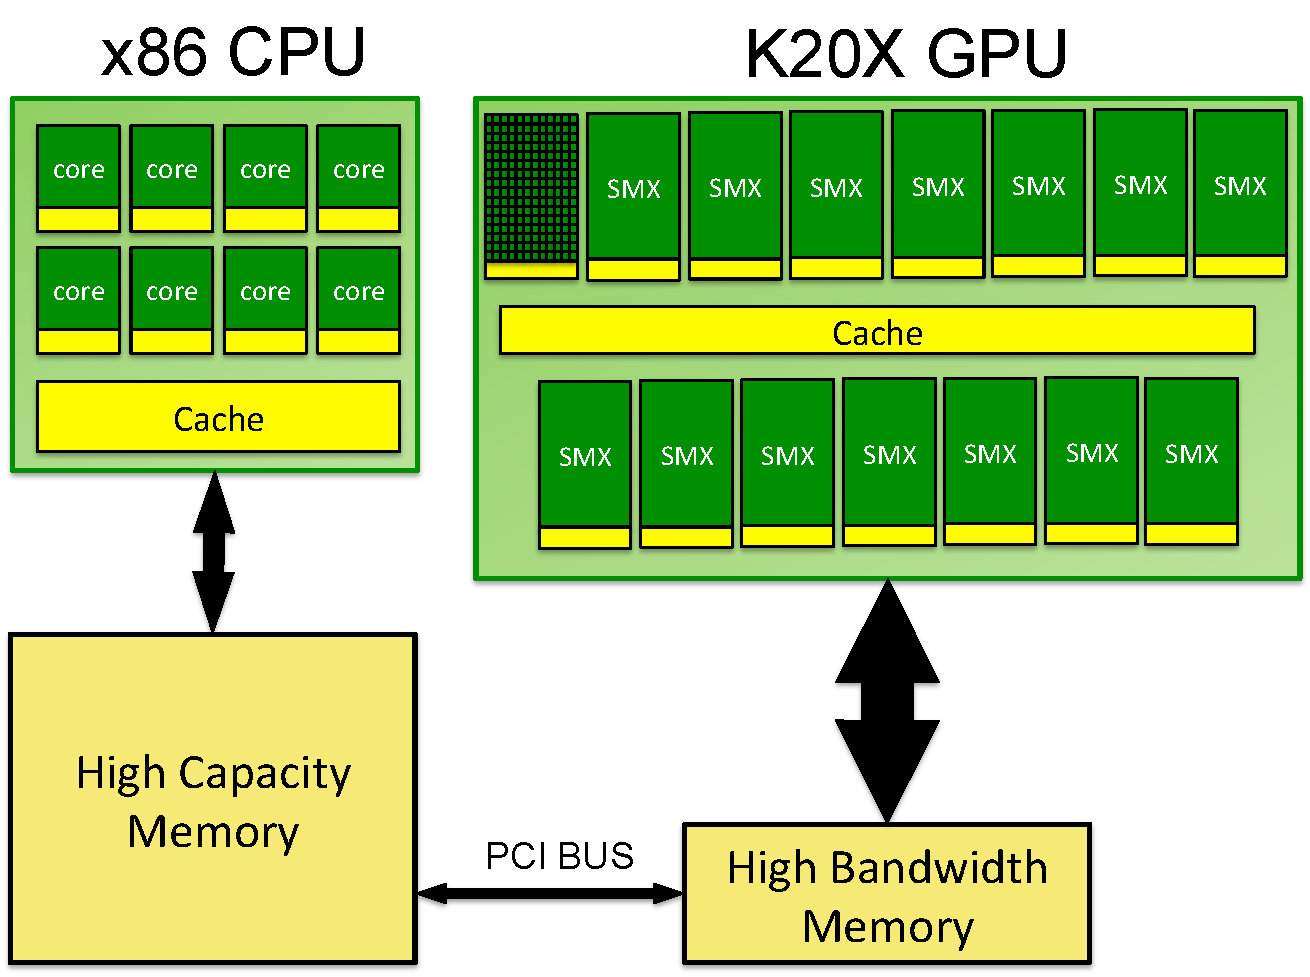
\includegraphics[width=0.9\textwidth]{./images/node.pdf}
    \end{center}
\end{frame}

%%%%%%%%%%%%%%%%%%%%%%%%%%%%%%%%%%%%
\begin{frame}[fragile]{}
%%%%%%%%%%%%%%%%%%%%%%%%%%%%%%%%%%%%
    \begin{info}{Host and device have separate memory spaces}
        \begin{itemize}
            \item data must be copied between host and device memory via PCI
            \item data must be in device memory for kernels to access
                \begin{itemize}
                    \item not strictly true\ldots
                    \item but a strict requirement for high performance
                \end{itemize}
            \item ensure data is in the right memory space \emph{before} computation starts
            \begin{itemize}
                \item PCIe2 = 6-12 GB/s
                \item CPU socket = 35-50 GB/s
                \item K20X  = 180 GB/s
            \end{itemize}
        \end{itemize}
    \end{info}

\end{frame}

%%%%%%%%%%%%%%%%%%%%%%%%%%%%%%%%%%%%
\begin{frame}[fragile]{}
%%%%%%%%%%%%%%%%%%%%%%%%%%%%%%%%%%%%
    \begin{info}{CUDA uses C pointers to reference GPU memory}
        \centering \lst{double *data = // pass an address to either host or device memory}
        \begin{itemize}
            \item a pointer can hold an address in \emph{either} device or host memory
            \item accessing a device pointer in host code, or vice versa, is \emph{undefined behaviour}
            \item we have to take care that we know which memory space a pointer is addressing
        \end{itemize}
        The CUDA runtime library provides functions that can be used to allocate, free and copy device memory
    \end{info}

\end{frame}

%%%%%%%%%%%%%%%%%%%%%%%%%%%%%%%%%%%%
\begin{frame}[fragile]{}
%%%%%%%%%%%%%%%%%%%%%%%%%%%%%%%%%%%%
    \begin{info}{Allocating device memory}
        \centering \lst{cudaMalloc(void **ptr, size_t size)}
    \begin{itemize}
        \item \lst{size} number of bytes to allocate
        \item \lst{ptr} points to allocated memory on exit
    \end{itemize}
    \end{info}

    \begin{info}{Freeing device memory}
        \centering \lst{cudaFree(void *ptr)}
    \end{info}

    \begin{code}{Allocate memory for 100 doubles on device}
%..................................
        \begin{lstlisting}[style=boxcuda]
double *v; // C pointer that will point to device memory
auto size_in_bytes = 100*sizeof(double);
cudaMalloc(&v, size_in_bytes); // allocate memory
cudaFree(v);                   // free memory
\end{lstlisting}
%..................................
    \end{code}
\end{frame}

%%%%%%%%%%%%%%%%%%%%%%%%%%%%%%%%%%%%
\begin{frame}[fragile]{}
%%%%%%%%%%%%%%%%%%%%%%%%%%%%%%%%%%%%
    \begin{info}{Perform blocking copy (host waits for copy to finish)}
        \centering \lst{cudaMemcpy(void *dst, void *src, size_t size, cudaMemcpyKind kind)}
    \begin{itemize}
        \item \lst{dst} destination pointer
        \item \lst{src} source pointer
        \item \lst{size} number of \emph{bytes} to copy to \lst{dst}
        \item \lst{kind} enumerated type specifying \emph{direction} of copy:
            \lst{cudaMemcpyHostToDevice}, also \lst{DeviceToHost}, \lst{DeviceToDevice}
    \end{itemize}
    \end{info}

    \begin{code}{Copy 100 doubles to device, then back to host}
%..................................
        \begin{lstlisting}[style=boxcuda]
int size = 100*sizeof(double); // size in bytes
double *v_d;
cudaMalloc(&v_d, size);              // allocate on device
double *v_h = (double*)malloc(size); // allocate on host
cudaMemcpy(v_d, v_h, size, cudaMemcpyHostToDevice);
cudaMemcpy(v_h, v_d, size, cudaMemcpyDeviceToHost);
\end{lstlisting}
%..................................
    \end{code}
\end{frame}

%%%%
\begin{frame}[fragile]{}

    \begin{info}{Errors happen\ldots}
        all API functions return error codes that indicate either:
        \begin{itemize}
            \item success
            \item an error in the API call
            \item an error in an earlier asynchronous call
        \end{itemize}
        the return value is the enum type \lst{cudaError_t}
        \begin{itemize}
            \item e.g. \lst{cudaError_t status = cudaMalloc(&v, 100);}
            \begin{itemize}
                \item status is \{\lst{cudaSuccess}, \lst{cudaErrorMemoryAllocation}\}
            \end{itemize}
        \end{itemize}
    \end{info}

    \begin{info}{Handling errors}
        \centering \lst{const char* cudaGetErrorString(status)}
        \begin{itemize}
            \item returns a string describing status
        \end{itemize}
        \centering \lst{cudaError_t cudaGetLastError()}
        \begin{itemize}
            \item returns the last error
            \item resets status to \lst{cudaSuccess}
        \end{itemize}
    \end{info}

\end{frame}

%%%%
\begin{frame}[fragile]{}

    \begin{code}{Copy 100 doubles to device \emph{with error checking}}
%..................................
        \begin{lstlisting}[style=boxcuda]
double *v_d;
int size = sizeof(double)*100;
double *v_host = (double*)malloc(size);
cudaError_t status = cudaMalloc(&v_d, size);
if(status != cudaSuccess) {
  printf("cuda error : %s\n", cudaGetErrorString(status));
  exit(1);
}
status =
  cudaMemcpy(v_d, v_h, size, cudaMemcpyHostToDevice);
if(status != cudaSuccess) {
  printf("cuda error : %s\n", cudaGetErrorString(status));
  exit(1);
}
        \end{lstlisting}
%..................................
    \end{code}

    \begin{info}{It is essential to test for errors}
        But it is tedious and obfuscates our source code
    \end{info}
\end{frame}

%%%%%%%%%%%%%%%%%%%%%%%%%%%%%%%%%%%%%%%%%%%%
\begin{frame}[fragile]{Exercise: API Basics}
%%%%%%%%%%%%%%%%%%%%%%%%%%%%%%%%%%%%%%%%%%%%
    Open \lst{cuda/exercises/util.h}
    \begin{enumerate}
        \item what does \lst{cuda_check_error()} do?

        \item look at the template wrappers \lst{malloc_host} and \lst{malloc_device}
        \begin{itemize}
            \item what do they do?
            \item what are the benefits over using \lst{cudaMalloc} and \lst{free} directly?
            \item do we need corresponding functions for \lst{cudaFree} and \lst{free}?
        \end{itemize}

        \item write a wrapper around \lst{cudaMemcpy} for copying data from host to device
        \begin{itemize}
            \item use the example for the reverse operation \lst{copy_device_to_host_sync}
            \item remember to check for errors!
        \end{itemize}

        \item compile the test and run
        \begin{itemize}
            %\item \lst{make axpy_cublas}
            \item it will pass with no errors on success
        \end{itemize}

    \vspace{-5pt}
\begin{lstlisting}[style=terminal]
make axpy_cublas
aprun ./axpy_cublas 8
\end{lstlisting}
    \end{enumerate}

\end{frame}


%% CHAPTER SLIDE
\cscschapter{Going Parallel : Kernels and Threads}

%%%%%%%%%%%%%%%%%%%%%%%%%%%%%%%%%%%%%%%%%%%%
\begin{frame}[fragile]{}
%%%%%%%%%%%%%%%%%%%%%%%%%%%%%%%%%%%%%%%%%%%%
    \begin{info}{Threads and kernels}
        \begin{itemize}
            \item \emph{threads} are streams of execution, run simultaneously on GPU (1000s)
            \item \emph{kernel} is the task run by each thread
            \item CUDA provides language support for
            \begin{itemize}
                \item writing kernels
                \item launching many threads to execute a kernel in parallel
            \end{itemize}
            \item CUDA hides the low-level details of launching threads
        \end{itemize}
    \end{info}
    \begin{info}{The process for porting to CUDA}
        \begin{enumerate}
            \item formulate algorithm in terms of parallel work items
            \item write a kernel implementing a work item on one thread
            \item launch the kernel with the required number of threads
        \end{enumerate}
    \end{info}

\end{frame}

%%%%%%%%%%%%%%%%%%%%%%%%%%%%%%%%%%%%%%%%%%%%
\begin{frame}[fragile]{}
%%%%%%%%%%%%%%%%%%%%%%%%%%%%%%%%%%%%%%%%%%%%
    \begin{info}{Scaled Vector Addition (\axpy)}
        The exercise in the first section used CUBLAS to perform scaled vector addition
            $$\mathbf{y} = \mathbf{y} + \alpha \mathbf{x}$$
            \vspace{-15pt}
        \begin{itemize}
            \item $\mathbf{x}$ and $\mathbf{y}$ are vectors of length $n$ \hfill $x,y \in \mathbb{R}^n$
            \item $\alpha$ is scalar \hfill $\alpha\in\mathbb{R}$
        \end{itemize}
        \axpy can be performed as $n$ \emph{independent} operations
        $$y_i \leftarrow y_i + a*x_i,\quad i = {0, 1, \dots, n-1}$$
        which can be performed independently and in any order
    \end{info}

    \begin{code}{\axpy implemented with for loop}
%..................................
        \begin{lstlisting}[style=boxcuda]
void axpy(double *y, double *x, double a, int n) {
  for(int i=0; i<n; ++i)
    y[i] = y[i] + a*x[i];
}
        \end{lstlisting}
%..................................
    \end{code}

\end{frame}

%%%%%%%%%%%%%%%%%%%%%%%%%%%%%%%%%%%%%%%%%%%%
\begin{frame}[fragile]{}
%%%%%%%%%%%%%%%%%%%%%%%%%%%%%%%%%%%%%%%%%%%%
    \begin{info}{What is a kernel?}
    \begin{itemize}
        \item a kernel defines the work item for a single thread
        \item the work is performed by many threads executing the same kernel \emph{simultaneously}
        \item Conceptually corresponds to the inner part of a loop for BLAS1 operations like \axpy
    \end{itemize}
    \end{info}

    \vspace{-10pt}
    \begin{columns}[T]
        \begin{column}{0.5\textwidth}
            \begin{codecolumn}{host : add two vectors}
%..................................
        \begin{lstlisting}[style=boxcudatiny]

void add_cpu(int *a, int *b, int n){
  for(auto i=0; i<n; ++i)
    a[i] = a[i] + b[i];
}
        \end{lstlisting}
%..................................
            \end{codecolumn}
        \end{column}
        \begin{column}{0.5\textwidth}
            \begin{codecolumn}{CUDA : add two vectors}
%..................................
        \begin{lstlisting}[style=boxcudatiny]
__global__
void add_gpu(int *a, int *b, int n){
  auto i = threadIdx.x;
  a[i] = a[i] + b[i];
}
        \end{lstlisting}
%..................................
            \end{codecolumn}
        \end{column}
    \end{columns}

    \vspace{-2pt}
    \begin{info}{}
    \begin{itemize}
        \item \lst{__global__} keyword indicates a kernel
        \item \lst{threadIdx} used to find unique id of each thread
    \end{itemize}
    \end{info}
\end{frame}

%%%%%%%%%%%%%%%%%%%%%%%%%%%%%%%%%%%%%%%%%%%%
\begin{frame}[fragile]{}
%%%%%%%%%%%%%%%%%%%%%%%%%%%%%%%%%%%%%%%%%%%%
    \begin{info}{launching a kernel}
    \begin{itemize}
        \item host code launches a kernel on the GPU \emph{asyncronously}
        \item CUDA provides special \lst{@<<<@_,_@>>>@} syntax for launching a kernel
        \begin{itemize}
            \item \lst{add_gpu@<<<@1, num_threads@>>>@(args... )} will launch the kernel \lst{add_gpu} with \lst{num_threads} parallel threads.
        \end{itemize}
    \end{itemize}
    \end{info}

    \begin{columns}[T]
        \begin{column}{0.5\textwidth}
            \begin{codecolumn}{host : add two vectors}
%..................................
        \begin{lstlisting}[style=boxcuda]
auto n = 1024;
auto a = host_malloc<int>(n);
auto b = host_malloc<int>(n);
add_cpu(a, b, n);
        \end{lstlisting}
%..................................
            \end{codecolumn}
        \end{column} \begin{column}{0.5\textwidth}
            \begin{codecolumn}{CUDA : add two vectors}
%..................................
        \begin{lstlisting}[style=boxcuda]
auto n = 1024;
auto a = device_malloc<int>(n);
auto b = device_malloc<int>(n);
add_gpu@<<<@1,n@>>>@(a, b, n);
        \end{lstlisting}
%..................................
            \end{codecolumn}
        \end{column}
    \end{columns}

\end{frame}

%%%%%%%%%%%%%%%%%%%%%%%%%%%%%%%%%%%%%%%%%%%%
\begin{frame}[fragile]{Exercise: My First Kernel}
%%%%%%%%%%%%%%%%%%%%%%%%%%%%%%%%%%%%%%%%%%%%
    Open \lst{cuda/exercises/axpy/axpy_kernel.cu}

    \begin{enumerate}
        \item Write a kernel that implements \axpy for \lst{double}
        \begin{itemize}
            \item \lst{axpy_kernel(double *y, double *x, double a, int n)}
            \item \extra can you write a C++ templated version for any type?
        \end{itemize}

        \item Replace the call to \lst{cublasDaxpy} with an invocation of your new kernel
        \item Compile the test and run
        \begin{itemize}
            \item it will pass with no errors on success
            \item first try with small vectors of size 8
            \item try increasing launch size... what happens?
        \end{itemize}
        \item \extra can you extend the kernel to work for larger arrays?
    \end{enumerate}
\end{frame}



%% CHAPTER SLIDE
\cscschapter{Scaling Up : Thread Blocks}

%%%%%%%%%%%%%%%%%%%%%%%%%%%%%%%%%%%%%%%%%%%%
\begin{frame}[fragile]{}
%%%%%%%%%%%%%%%%%%%%%%%%%%%%%%%%%%%%%%%%%%%%
    \begin{info}{}
        In the \axpy exercises we were limited to 1024 threads for a kernel launch
        \begin{itemize}
            \item but we need to scale beyond 1024 threads for the \emph{massive parallelism} we were promised!
        \end{itemize}
    \end{info}

    \begin{info}{Thread blocks and grids}
        kernels are executed in groups of threads called \emph{thread blocks}
        \vspace{-12pt}
        \begin{itemize}
            \item the launch configuration \lst{axpy@<<<@grid_dim, block_dim@>>>@(...)}
            \begin{itemize}
                \item launch a \emph{grid} of \lst{grid_dim} \emph{blocks}
                \item each \emph{block} has \lst{block_dim} \emph{threads}
                \item for a total of \lst{grid_dim}$\times$\lst{block_dim} threads
            \end{itemize}
            \item previously we launched just one thread block \lst{axpy@<<<@1, n@>>>@(...)}
        \end{itemize}
    \end{info}

\end{frame}

%%%%%%%%%%%%%%%%%%%%%%%%%%%%%%%%%%%%%%%%%%%%
\begin{frame}[fragile]{}
%%%%%%%%%%%%%%%%%%%%%%%%%%%%%%%%%%%%%%%%%%%%
    \begin{info}{Why the additional complexity of grids+blocks+threads?}
        \centering \emph{Because coordination between threads doesn't scale}
        \begin{itemize}
            \item threads in a block can synchronize and share resources
            \item this does not scale past a certain number of cores/threads
            \item on the K20X GPU streaming multiprocessor (SMX) has 192 CUDA cores, and can run 2028 threads
            \item threads in a block run on the same SMX, with shared resources and thread cooperation
            \item work is broken into blocks, which are distributed over the 14 SMXs in the K20X GPU
        \end{itemize}
    \end{info}
\end{frame}

%%%%%%%%%%%%%%%%%%%%%%%%%%%%%%%%%%%%%%%%%%%%
\begin{frame}[fragile]{}
%%%%%%%%%%%%%%%%%%%%%%%%%%%%%%%%%%%%%%%%%%%%
\begin{center}
\vspace{-0.75cm}
\begin{tabular}{|c|m{4cm}|m{5cm}|}
    \cline{1-2}
        concept & hardware &  \multicolumn{1}{c}{} \\
    \hline
        thread &
        \begin{minipage}{4cm}
            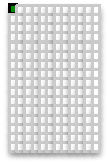
\includegraphics[width=0.3\textwidth]{./images/core.pdf}
        \end{minipage} &
        \footnotesize
        \begin{itemize}
            \item each thread executed on one core
        \end{itemize} \\
    \hline
        block &
        \begin{minipage}{4cm}
            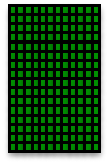
\includegraphics[width=0.3\textwidth]{./images/smx.pdf}
        \end{minipage} &
        \footnotesize
        \begin{itemize}
            \item block executed on 1 SMX
            \item multiple blocks per SMX if sufficient resources
            \item threads in a block share SMX resources
        \end{itemize} \\
    \hline
        grid &
        \begin{minipage}{4cm}
            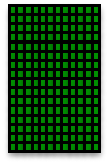
\includegraphics[width=0.3\textwidth]{./images/smx.pdf}
            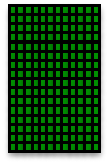
\includegraphics[width=0.3\textwidth]{./images/smx.pdf}
            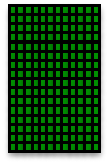
\includegraphics[width=0.3\textwidth]{./images/smx.pdf}
        \end{minipage} &
        \footnotesize
        \begin{itemize}
            \item kernel is executed in grid of blocks
            \item blocks distributed over SMXs
            \item multiple kernels can run at same time
        \end{itemize} \\
\hline
\end{tabular}
\end{center}
\end{frame}

%%%%%%%%%%%%%%%%%%%%%%%%%%%%%%%%%%%%%%%%%%%%
\begin{frame}[fragile]{}
%%%%%%%%%%%%%%%%%%%%%%%%%%%%%%%%%%%%%%%%%%%%
    \begin{info}{Calculating thread indexes}
        A kernel has to calculate the index of its work item
        \begin{itemize}
            \item in \lst{axpy} we used \lst{threadIdx.x} for the index
            \item when using multiple blocks, we need more information, which is available in the following \emph{magic variables}:
        \end{itemize}

        \begin{center}
            \begin{tabular}{ll}
            \lst{gridDim}   &: total number of blocks in the grid \\
            \lst{blockDim}  &: number of threads in a thread block \\
            \lst{blockIdx}  &: index of block \lst{[0, gridDim-1]} \\
            \lst{threadIdx} &: index of thread in thread block \lst{[0, blockDim-1]} \\
            \end{tabular}
        \end{center}

    \end{info}
\end{frame}

%%%%%%%%%%%%%%%%%%%%%%%%%%%%%%%%%%%%%%%%%%%%
\begin{frame}[fragile]{}
%%%%%%%%%%%%%%%%%%%%%%%%%%%%%%%%%%%%%%%%%%%%
    \begin{info}{Calculating thread indexes}
        Consider accessing an array of length 24 with 8 threads per block. The \emph{dimensions} of the kernel launch are:
        \begin{itemize}
            \item \lst{blockDim.x == 8} (8 threads/block)
            \item \lst{gridDim.x == 3} (3 blocks)
        \end{itemize}
        We calculate the index for our thread using the formula
        \begin{center}
            \lst{auto index = threadIdx.x + blockIdx.x*blockDim.x}\\
            \vspace{0.5cm}
            \centering 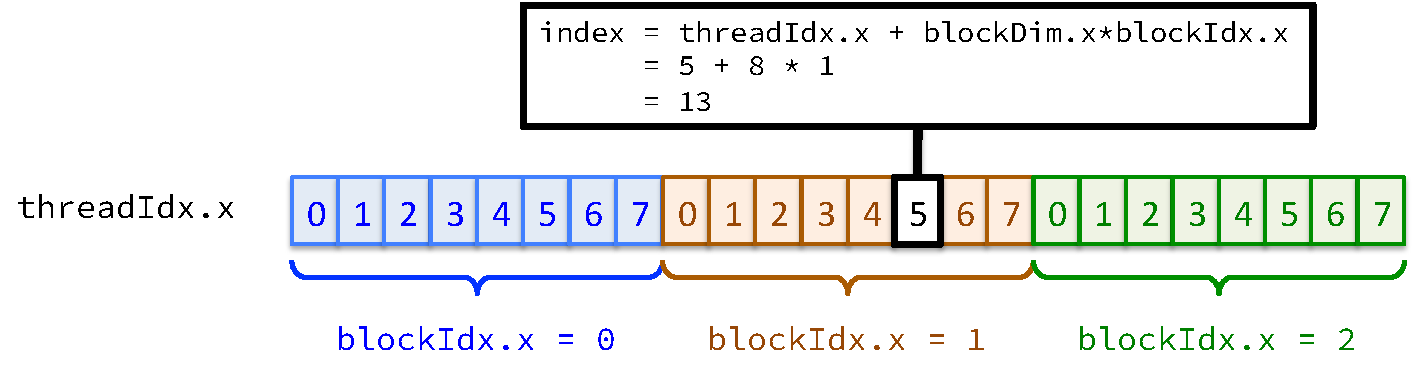
\includegraphics[width=\textwidth]{./images/blocks.pdf}
        \end{center}
    \end{info}
\end{frame}

%%%%%%%%%%%%%%%%%%%%%%%%%%%%%%%%%%%%%%%%%%%%
\begin{frame}[fragile]{}
%%%%%%%%%%%%%%%%%%%%%%%%%%%%%%%%%%%%%%%%%%%%
    \begin{info}{Calculating grid dimensions}
            The number of thread blocks and the number of threads per block are parameters for the kernel launch:
            \begin{center}
                \lst{kernel@<<<@blocks, threads_per_block@>>>@(...)}
            \end{center}
            Remember to guard against overflow when the number of work items is not divisible by the thread block size
    \end{info}

    \begin{code}{vector addition with multiple blocks}
%..................................
        \begin{lstlisting}[style=boxcudatiny]
__global__
void add_gpu(int *a, int *b, int n){
  auto i = threadIdx.x + blockIdx.x*blockDim.x;
  if(i<n) { // guard against access off end of arrays
    a[i] += b[i];
  }
}

// in main()
auto block_size = 512;
auto num_blocks = (n + (block_size-1)) / block_size;
add_gpu@<<<@num_blocks, block_size@>>>@(a, b, n);
        \end{lstlisting}
%..................................
    \end{code}
\end{frame}

%%%%%%%%%%%%%%%%%%%%%%%%%%%%%%%%%%%%%%%%%%%%
\begin{frame}[fragile]{}
%%%%%%%%%%%%%%%%%%%%%%%%%%%%%%%%%%%%%%%%%%%%
    \begin{info}{Calculating grid dimensions}
        We have to take care when calculating the number of blocks in the grid, i.e. \lst{blocks}:
        \begin{center}
            \lst{kernel@<<<@blocks, threads_per_block@>>>@(...)}
        \end{center}
        Most likely, the number of work items \lst{n} is not a multiple of \lst{threads_per_block}.
        \begin{itemize}
            \item in which case some threads in the last thread block will do any work
        \end{itemize}
    \end{info}

    \begin{code}{Calculating grid dimensions}
%..................................
        \begin{lstlisting}[style=boxcudatiny]
// in main()
auto block_size = 512;
auto num_blocks = (n + (block_size-1)) / block_size;
add_gpu@<<<@num_blocks, block_size@>>>@(a, b, n);
        \end{lstlisting}
%..................................
    \end{code}
\end{frame}

%%%%%%%%%%%%%%%%%%%%%%%%%%%%%%%%%%%%%%%%%%%%
\begin{frame}[fragile]{}
%%%%%%%%%%%%%%%%%%%%%%%%%%%%%%%%%%%%%%%%%%%%
    \begin{info}{The number of threads per block impacts performance}
    \begin{itemize}
        \item the optimal number depends on the resources (registers, shared memory, etc) that a kernel requires
    \end{itemize}
    \end{info}

    \begin{code}{Choosing block size automatically (CUDA 6.5 and later)}
%..................................
        \begin{lstlisting}[style=boxcudatiny]
int block_size, min_grid_dim;

cudaOccupancyMaxPotentialBlockSize(&min_grid_size, &block_size,
                                   add_gpu, 0, n);
auto num_blocks = (n + (block_size-1)) / block_size;

add_gpu@<<<@num_blocks, block_size@>>>@(a, b, n);
        \end{lstlisting}
%..................................
    \end{code}

    \begin{info}{}
    The variable \lst{min_grid_size} is set to the minimum number of blocks required to \emph{saturate} the GPU, i.e. provide the GPU with enough work to utilize all of the SMXs.
    \end{info}
\end{frame}

%%%%%%%%%%%%%%%%%%%%%%%%%%%%%%%%%%%%%%%%%%%%
\begin{frame}[fragile]{Exercise: Blocks}
%%%%%%%%%%%%%%%%%%%%%%%%%%%%%%%%%%%%%%%%%%%%
    Open \lst{cuda/exercises/axpy/axpy.cu} from the last exercise
    \begin{enumerate}
        \item Extend the \axpy kernel for arbitrarily large input arrays (any \lst{n})

        \item Update the call site to calculate the grid configuration

        \item Compile the test and run
        \begin{itemize}
            \item it will pass with no errors on success
        \end{itemize}

        \item Experiment with varying the size of the arrays (scaling)
        \begin{itemize}
            \item start small and increase
        \end{itemize}

        \item finish the \lst{newton.cu} example
        \begin{itemize}
            \item how do the h2d, d2h and kernel timings compare?
        \end{itemize}

        \item \extra Compare scaling with the \lst{axpy_omp} benchmark

        \item \extra Experiment with varying the block size
        \begin{itemize}
            \item try \lst{cudaOccupancyMaxPotentialBlockSize}.
        \end{itemize}

    \end{enumerate}

\end{frame}

%%%%%%%%%%%%%%%%%%%%%%%%%%%%%%%%%%%%%%%%%%%%
\begin{frame}[fragile]{Exercise: Results}
%%%%%%%%%%%%%%%%%%%%%%%%%%%%%%%%%%%%%%%%%%%%

%\begin{tikzpicture}
%    \pgfplotsset{footnotesize}
%    \begin{semilogyaxis}[
%        height=0.7\textwidth,
%        width=\textwidth,
%        xmin=8,xmax=28,
%        xtick={8,12,16,20,24,28},
%        xlabel=$log_2(n)$,
%        ylabel=time (s),
%        legend style = {at={(0.05,0.95)}, anchor=north west},
%        every axis y label/.style=
%            {at={(ticklabel cs:0.5)},rotate=90,anchor=near ticklabel},
%        grid=major]
%        \addplot[color=blue,mark=*]  table[x=n,y=gpu]  {./plots/axpy.tbl};
%        \addplot[color=red,mark=*]   table[x=n,y=omp1] {./plots/axpy.tbl};
%        \addplot[color=green,mark=*] table[x=n,y=omp8] {./plots/axpy.tbl};
%        \legend{CUDA, OpenMP 1, OpenMP 8};
%    \end{semilogyaxis}
%\end{tikzpicture}

\begin{center}
\begin{tikzpicture}
    \pgfplotsset{footnotesize}
    \begin{axis}[
        height=0.4\textwidth,
        width=\textwidth,
        xmin=8,xmax=28,
        ymin=0,ymax=6,
        xtick={8,12,16,20,24,28},
        ytick={0,1,2,3,4,5,6},
        xlabel=$log_2(n)$,
        ylabel=speedup,
        legend style = {at={(0.05,0.95)}, anchor=north west},
        every axis y label/.style=
            {at={(ticklabel cs:0.5)},rotate=90,anchor=near ticklabel},
        grid=major]
        \addplot[color=blue,mark=*]  table[x=n,y expr=\thisrow{omp8}/\thisrow{gpu}]  {./plots/axpy.tbl};
        \addplot[color=black,mark=*] table[x=n,y expr=\thisrow{omp8}/\thisrow{omp8}] {./plots/axpy.tbl};
        \legend{CUDA speedup, OpenMP 8 thread};
    \end{axis}
\end{tikzpicture}
\end{center}

The GPU is a throughput device:
\begin{itemize}
\item the CUDA implementation is faster for $2^{15}\approx32,000$
\item requires $2^{20}\approx1,000,000$ to get ``advertised'' $5\times$ speedup
\end{itemize}
You have to provide enough parallelism to exploit many cores

\end{frame}

% cudaOccupancyMaxPotentialBlockSize suggests block_dim 256-1024, depending on n
% in practice it makes little difference


%%++++++++++++++++++++++++++++++++
\cscschapter{Cooperating Threads}
%++++++++++++++++++++++++++++++++

%%%%%%%%%%%%%%%%%%%%%%%%%%%%%%%%%%%%%%%%%%%%
\begin{frame}[fragile]{}
%%%%%%%%%%%%%%%%%%%%%%%%%%%%%%%%%%%%%%%%%%%%
    \centering
    Most algorithms do not lend themselves to trivial parallelization

%----------------------------
    \begin{code}{reductions : e.g. dot product}
        \begin{lstlisting}[style=boxcudatiny]
int dot(int *x, int *y, int n){
  int sum = 0.;
  for(auto i=0; i<n; ++i)
    sum += x[i]*y[i];
  return sum;
}
        \end{lstlisting}
    \end{code}
%----------------------------
\vspace{-7pt}
%----------------------------
        \begin{code}{scan : e.g. prefix sum}
            \begin{lstlisting}[style=boxcudatiny]
void prefix_sum(int *x, int n){
  for(auto i=1; i<n; ++i)
    x[i] += x[i-1];
}
        \end{lstlisting}
    \end{code}
%----------------------------
\vspace{-7pt}
%----------------------------
    \begin{code}{fusing piplined stencil loops : e.g. apply blur kernel twice}
        \begin{lstlisting}[style=boxcudatiny]
void twice_blur(float *in, float *out, int n){
  float buff[n];
  for(auto i=1; i<n-1; ++i)
    buff[i] = 0.25f*(in[i-1]+in[i+1]+2f*in[i]);
  for(auto i=2; i<n-2; ++i)
    out[i] = 0.25f*(buff[i-1]+buff[i+1]+2f*buff[i]);
}
        \end{lstlisting}
    \end{code}

\end{frame}

%%%%%%%%%%%%%%%%%%%%%%%%%%%%%%%%%%%%%%%%%%%%
\begin{frame}[fragile]{}
%%%%%%%%%%%%%%%%%%%%%%%%%%%%%%%%%%%%%%%%%%%%
    \begin{columns}[T]
        \begin{column}{0.3\textwidth}
            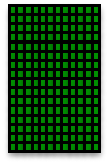
\includegraphics[width=\textwidth]{./images/smx.pdf}
        \end{column}

        \begin{column}{0.7\textwidth}
            \begin{info}{Block-Level synchronization}
            CUDA provides mechanisms for cooperation between \emph{threads in a thread block}.
            \begin{itemize}
                \item All threads in a block run on the same SMX
                \item Resources for synchronization are at SMX level
                \item No synchronization between blocks
            \end{itemize}
            \end{info}
        \end{column}
    \end{columns}

\end{frame}

%%%%%%%%%%%%%%%%%%%%%%%%%%%%%%%%%%%%%%%%%%%%
\begin{frame}[fragile]{}
%%%%%%%%%%%%%%%%%%%%%%%%%%%%%%%%%%%%%%%%%%%%
    %\begin{info}{}
        Cooperation between threads requires sharing of data
        \begin{itemize}
            \item All threads in a block can share data using \emph{shared memory}
            \item Shared memory is \emph{not visible} to threads in other thread blocks
        \end{itemize}
    %\end{info}

\end{frame}

%%%%%%%%%%%%%%%%%%%%%%%%%%%%%%%%%%%%%%%%%%%%
\begin{frame}[fragile]{}
%%%%%%%%%%%%%%%%%%%%%%%%%%%%%%%%%%%%%%%%%%%%
    \begin{info}{One-dimensional blur kernel}
        \centering $\text{out}_i \leftarrow 0.25(\text{in}_{i-1}+2\text{in}_i+\text{in}_{i+1})$
        \begin{itemize}
            \item each output value is a linear combination of neighbours in input array
            \item first we look at naiive implementation
        \end{itemize}
    \end{info}

    \begin{code}{Host implementation of blur kernel}
        \begin{lstlisting}[style=boxcudatiny]
void blur(double *in, double *out, int n){
  float buff[n];
  for(auto i=1; i<n-1; ++i)
    out[i] = 0.25*(2*in[i]+in[i-1]+in[i+1]);
}
        \end{lstlisting}
    \end{code}

\end{frame}

%%%%%%%%%%%%%%%%%%%%%%%%%%%%%%%%%%%%%%%%%%%%
\begin{frame}[fragile]{}
%%%%%%%%%%%%%%%%%%%%%%%%%%%%%%%%%%%%%%%%%%%%
    \begin{center}
        Our first CUDA implementation of the blur kernel has each thread load the three values required to form its output
    \end{center}
    \begin{code}{First implementation of blur kernel}
        \begin{lstlisting}[style=boxcudatiny]
__global__ void
blur(const double *in, double* out, int n) {
  int i = threadIdx.x + 1; // assume one thread block

  if(i<n-1) {
    out[i] = 0.25*(in[i-1] + 2*in[i] + in[i+1]);
  }
}
        \end{lstlisting}
    \end{code}

\end{frame}

%%%%%%%%%%%%%%%%%%%%%%%%%%%%%%%%%%%%%%%%%%%%
\begin{frame}[fragile]{}
%%%%%%%%%%%%%%%%%%%%%%%%%%%%%%%%%%%%%%%%%%%%
    \centering
    Each thread has to load 3 values from global memory to calculate its output \\
    \includegraphics[width=0.8\textwidth]{./images/blur_point_gather.pdf} \\
    Alternatively, each value in the input array has to be loaded 3 times \\
    \includegraphics[width=0.8\textwidth]{./images/blur_point_scatter.pdf} \\
\end{frame}

%%%%%%%%%%%%%%%%%%%%%%%%%%%%%%%%%%%%%%%%%%%%
\begin{frame}[fragile]{}
%%%%%%%%%%%%%%%%%%%%%%%%%%%%%%%%%%%%%%%%%%%%
    To take advantage of shared memory the kernel is split into two stages:
    \begin{enumerate}
        \item load \lst{in[i]} into shared memory \lst{buffer[i]}
        \begin{itemize}
            \item one thread has to load \lst{in[0]} \& \lst{in[n]}
        \end{itemize}
        \item use values \lst{buffer[i-1:i+1]} to compute kernel
    \end{enumerate}

    \begin{center}
        \includegraphics[width=0.8\textwidth]{./images/blur_point_shared.pdf}
    \end{center}
\end{frame}

%%%%%%%%%%%%%%%%%%%%%%%%%%%%%%%%%%%%%%%%%%%%
\begin{frame}[fragile]{}
%%%%%%%%%%%%%%%%%%%%%%%%%%%%%%%%%%%%%%%%%%%%
    \begin{code}{Blur kernel with shared memory}
        \begin{lstlisting}[style=boxcudatiny]
__global__
void blur_shared_block(double *in, double* out, int n) {
    extern __shared__ double buffer[];

    auto i = threadIdx.x + 1;

    if(i<n-1) {
        // load shared memory
        buffer[i] = in[i];
        if(i==1) {
            buffer[0] = in[0];
            buffer[n] = in[n];
        }

        __syncthreads();

        out[i] = 0.25*(buffer[i-1] + 2.0*buffer[i] + buffer[i+1]);
    }
}
        \end{lstlisting}
    \end{code}

\end{frame}

%%%%%%%%%%%%%%%%%%%%%%%%%%%%%%%%%%%%%%%%%%%%
\begin{frame}[fragile]{}
%%%%%%%%%%%%%%%%%%%%%%%%%%%%%%%%%%%%%%%%%%%%
    \begin{info}{Declaring shared memory}
        \centering \lst{extern __shared__ double buffer[];}
        \begin{itemize}
            \item the size of memory to be allocated is specified when the kernel is launched
        \end{itemize}
    \end{info}

    \begin{info}{Synchronizing threads}
        \centering \lst{__syncthreads();}
        \begin{itemize}
            \item threads wait for all threads in thread block to finish loading shared memory buffer
            \item thread $i$ needs to wait for threads $i-1$ and $i+1$ to load values into \lst{buffer}
            \item synchronization required to avoid race conditions
            \begin{itemize}
                \item threads have to wait for other threads to fill \lst{buffer}
            \end{itemize}
        \end{itemize}
    \end{info}

\end{frame}

%%%%%%%%%%%%%%%%%%%%%%%%%%%%%%%%%%%%%%%%%%%%
\begin{frame}[fragile]{}
%%%%%%%%%%%%%%%%%%%%%%%%%%%%%%%%%%%%%%%%%%%%
    \begin{info}{Launching kernels with shared memory}
        An additional parameter is added to the launch syntax\\
        \centering \lst{blur@<<<@grid_dim, block_dim, shared_size@>>>@(...);}
        \begin{itemize}
            \item \lst{shared_size} is the shared memory \emph{in bytes} to be allocated \emph{per thread block}
        \end{itemize}
    \end{info}

    \begin{code}{Launch blur kernel with shared memory}
        \begin{lstlisting}[style=boxcudatiny]
__global__
void blur_shared(double *in, double* out, int n) {
  extern __shared__ double buffer[];

  int i = threadIdx.x + 1;
  // ...
}

// in main()
auto block_dim = n-2;
auto size_in_bytes = n*sizeof(double);

blur_shared@<<<@1, block_dim, size_in_bytes@>>>@(x0, x1, n);
        \end{lstlisting}
    \end{code}

\end{frame}

%%%%%%%%%%%%%%%%%%%%%%%%%%%%%%%%%%%%%%%%%%%%
\begin{frame}[fragile]{}
%%%%%%%%%%%%%%%%%%%%%%%%%%%%%%%%%%%%%%%%%%%%
    \begin{info}{Is it worth it?}
        A version of the blur kernel for arbitrarily large $n$ is provided in \lst{blur.cu} in the example code. The implementation is a bit awkward:
        \begin{itemize}
            \item  The \lst{in} and \lst{out} arrays use global indexes
            \item  The shared memory uses thread block local indexes
        \end{itemize}
        The \textasciitilde10\% performance improvement might be worth it, depending on how important the kernel is to overall application performance
    \end{info}

\end{frame}

%%%%%%%%%%%%%%%%%%%%%%%%%%%%%%%%%%%%%%%%%%%%
\begin{frame}[fragile]{}
%%%%%%%%%%%%%%%%%%%%%%%%%%%%%%%%%%%%%%%%%%%%
    \begin{info}{Buffering with shared memory}
        Shared memory is important for caching intermediate results used in pipelined operations
        \begin{itemize}
            \item shared memory is an order of magnitude faster than global DRAM
            \item by \emph{fusing} pipelined operations in one kernel, intermediate results can be stored in shared memory
            \item similar to blocking and tiling for cache
        \end{itemize}
    \end{info}


    \begin{code}{Double blur: basic OpenMP}
        \begin{lstlisting}[style=boxcudatiny]
void blur_twice(const double* in , double* out , int n) {
  static double* buffer = malloc_host<double>(n);

  #pragma omp parallel for
  for(auto i=1; i<n-1; ++i) {
    buffer[i] = 0.25*( in[i-1] + 2.0*in[i] + in[i+1]);
  }
  #pragma omp parallel for
  for(auto i=2; i<n-2; ++i) {
    out[i] = 0.25*( buffer[i-1] + 2.0*buffer[i] + buffer[i+1]);
  }
}
        \end{lstlisting}
    \end{code}

\end{frame}

%%%%%%%%%%%%%%%%%%%%%%%%%%%%%%%%%%%%%%%%%%%%
\begin{frame}[fragile]{}
%%%%%%%%%%%%%%%%%%%%%%%%%%%%%%%%%%%%%%%%%%%%
    %For a host implementation break work into blocks, to keep intermediate results in \lst{buffer} in cache.
    \begin{code}{Double blur: OpenMP with blocking for cache}
        \begin{lstlisting}[style=boxcudatiny]
void blur_twice(const double* in , double* out , int n) {
  auto const block_size = std::min(512, n-4);
  auto const num_blocks = (n-4)/block_size;
  static double* buffer = malloc_host<double>((block_size+4)*omp_get_max_threads());

  auto blur = [] (int pos, const double* u) {
    return 0.25*( u[pos-1] + 2.0*u[pos] + u[pos+1]);
  };

  #pragma omp parallel for
  for(auto b=0; b<num_blocks; ++b) {
    auto tid = omp_get_thread_num();
    auto first = 2 + b*block_size;
    auto last = first + block_size;

    auto buff = buffer + tid*(block_size+4);
    for(auto i=first-1, j=1; i<(last+1); ++i, ++j) {
      buff[j] = blur(i, in);
    }
    for(auto i=first, j=2;   i<last;   ++i, ++j) {
      out[i] = blur(j, buff);
    }
  }
}
        \end{lstlisting}
    \end{code}
\end{frame}

%%%%%%%%%%%%%%%%%%%%%%%%%%%%%%%%%%%%%%%%%%%%
\begin{frame}[fragile]{}
%%%%%%%%%%%%%%%%%%%%%%%%%%%%%%%%%%%%%%%%%%%%
    \begin{code}{double blur: CUDA with shared memory}
        \begin{lstlisting}[style=boxcudatiny]
__global__ void blur_twice(const double *in, double* out, int n) {
  extern __shared__ double buffer[];

  auto block_start = blockDim.x * blockIdx.x;
  auto block_end   = block_start + blockDim.x;
  auto lid = threadIdx.x + 2;
  auto gid = lid + block_start;

  auto blur = [] (int pos, double const* field) {
    return 0.25*(field[pos-1] + 2.0*field[pos] + field[pos+1]);
  };

  if(gid<n-2) {
    buffer[li] = blur(gi, in);
    if(threadIdx.x==0) {
        buffer[1]            = blur(block_start+1, in);
        buffer[blockDim.x+2] = blur(block_end+2, in);
    }

    __syncthreads();

    out[gi] = blur(li, buffer);
  }
}
        \end{lstlisting}
    \end{code}
\end{frame}

%%%%%%%%%%%%%%%%%%%%%%%%%%%%%%%%%%%%%%%%%%%%
\begin{frame}[fragile]{}
%%%%%%%%%%%%%%%%%%%%%%%%%%%%%%%%%%%%%%%%%%%%
    \begin{info}{Fused loop results}
        The OpenMP cache-aware version was harder to implement than the shared-memory CUDA version
        \begin{itemize}
            \item CUDA is harder to start because it makes us to think in parallel always
        \end{itemize}
        Both implementations benefit significantly from optimizations for fast on chip memory
    \end{info}
    \begin{columns}[T]
        \begin{column}{0.5\textwidth}
            \centering
            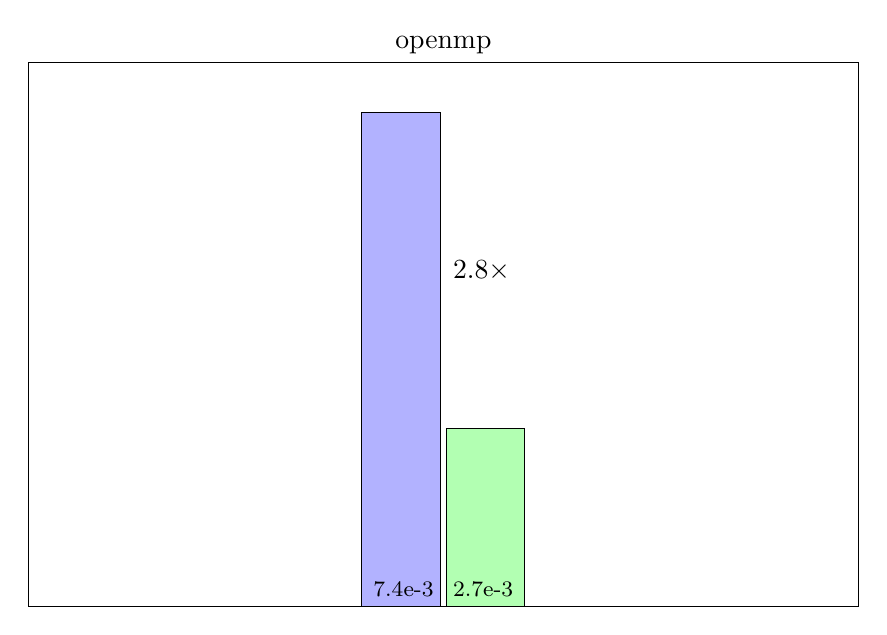
\begin{tikzpicture}
                \begin{axis}[
                    ybar,
                    height=0.7\textwidth,
                    width=\textwidth,
                    ymin=0,
                    ticks=none,
                    title={openmp},
                    title style={yshift=-1.5ex}
                ]
                \addplot
                    [draw=black, fill=blue!30, bar width=1cm]
                    coordinates {(1,7.37e-3)};
                \addplot
                    [draw=black, fill=green!30, bar width=1cm]
                    coordinates {(1,2.66e-3)};
                \node[right] at (axis cs:1,0.005) {2.8$\times$};
                \node[above left] at (axis cs:1,0) {\footnotesize7.4e-3};
                \node[above right] at (axis cs:1,0) {\footnotesize2.7e-3};
                %\legend{\tiny na\"ive, \tiny optimized};
                \end{axis}
            \end{tikzpicture}
        \end{column}

        \begin{column}{0.5\textwidth}
            \centering
            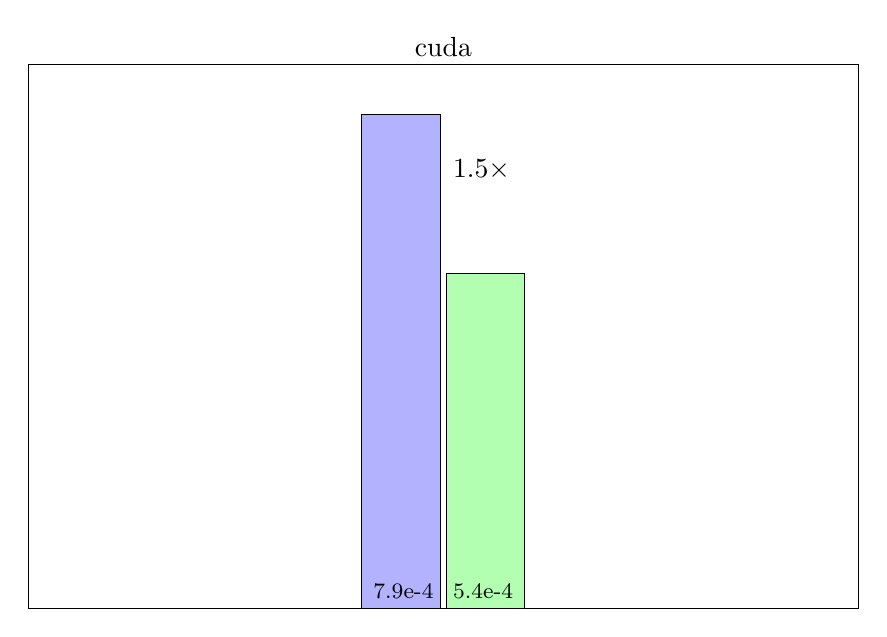
\begin{tikzpicture}
                \begin{axis}[
                    ybar,
                    height=0.7\textwidth,
                    width=\textwidth,
                    ymin=0,
                    ticks=none,
                    title={cuda},
                    title style={yshift=-1.5ex}
                ]

                \addplot
                   [draw=black, fill=blue!30, bar width=1cm]
                    coordinates {(1,7.89e-4)};
                \addplot
                   [draw=black, fill=green!30, bar width=1cm]
                    coordinates {(1,5.35e-4)};
                \node[right] at (axis cs:1,0.0007) {1.5$\times$};
                \node[above left] at (axis cs:1,0) {\footnotesize7.9e-4};
                \node[above right] at (axis cs:1,0) {\footnotesize5.4e-4};
                %\legend{\tiny na\"ive, \tiny optimized};
                \end{axis}
            \end{tikzpicture}
        \end{column}
    \end{columns}



\end{frame}

%%%%%%%%%%%%%%%%%%%%%%%%%%%%%%%%%%%%%%%%%%%%
\begin{frame}[fragile]{}
%%%%%%%%%%%%%%%%%%%%%%%%%%%%%%%%%%%%%%%%%%%%
    \begin{info}{CPU : optimizing for on-chip memory}
        \begin{itemize}
            \item Let hardware prefetcher automatically manage cache
            \item Choose block/tile sizes so that intermediate data will fit in a target cache (L1, L2 or L3)
        \end{itemize}
    \end{info}
    \begin{info}{GPU : optimizing for on-chip memory}
        \begin{itemize}
            \item Manage shared memory manually
            \begin{itemize}
                \item more control
                \item hardware-specific
            \end{itemize}
            \item Choose thread block sizes so that intermediate data will fit into shared memory on an SMX
        \end{itemize}
    \end{info}

\end{frame}

%%%%%%%%%%%%%%%%%%%%%%%%%%%%%%%%%%%%%%%%%%%%
\begin{frame}[fragile]{Exercise: Shared Memory}
%%%%%%%%%%%%%%%%%%%%%%%%%%%%%%%%%%%%%%%%%%%%
    Your task is to implement dot product in CUDA in \lst{cuda/exercises/dot.cu}.
    \begin{itemize}
        \item the host version has been implemented as \lst{dot_host()}
        \item assume that $n$ is a power of 2 and $n\leq1024$
    \end{itemize}

    Extensions :
    \begin{enumerate}
        \item can you make it work for arbitrary $n<1024$?
        \item how would you extend it to work for arbitrarily large $n$?
    \end{enumerate}

    \centering \includegraphics[width=0.5\textwidth]{./images/reduction.pdf}

\end{frame}

%++++++++++++++++++++++++++++++++
\cscschapter{Concurrency}
%++++++++++++++++++++++++++++++++

%%%%%%%%%%%%%%%%%%%%%%%%%%%%%%%%%%%%%%%%%%%%
\begin{frame}[fragile]{}
%%%%%%%%%%%%%%%%%%%%%%%%%%%%%%%%%%%%%%%%%%%%
    \begin{info}{Concurrency}
        \emph{Concurrency} is the ability to perform multiple CUDA operations simultaneously
        \begin{itemize}
            \item CUDA kernels
            \item copying from host to device
            \item copying from device to host
            \item operations on the host CPU
        \end{itemize}
    \end{info}

    \begin{info}{Concurrency enables}
        \begin{itemize}
            \item both CPU and GPU can work at the same time
            \item multiple tasks can be run on GPU simultaneously
            \item overlapping of communication and computation
        \end{itemize}
    \end{info}

\end{frame}

%%%%%%%%%%%%%%%%%%%%%%%%%%%%%%%%%%%%%%%%%%%%
\begin{frame}[fragile]{}
%%%%%%%%%%%%%%%%%%%%%%%%%%%%%%%%%%%%%%%%%%%%
    \begin{columns}[T]
        \begin{column}{0.5\textwidth}
            \begin{codecolumn}{Host code}
                \begin{lstlisting}[style=boxcudatiny]
kernel_1@<<<@...@>>>@(...);
kernel_2<@<<.@..@>>>@(...);
host_1(...);
host_2(...);
                \end{lstlisting}
            \end{codecolumn}
            %\begin{info}{CPU and GPU are asynchronous}
                The host:
                \begin{itemize}
                    \item launches the two CUDA kernels
                    \item then executes host calls sequentially 
                \end{itemize}
                The GPU:
                \begin{itemize}
                    \item executes asynchronously to host
                    \item executes kernels sequentially
                \end{itemize}
            %\end{info}
        \end{column}
        \begin{column}{0.5\textwidth}
            \includegraphics[width=\textwidth]{./images/async_null.pdf}
        \end{column}
    \end{columns}
\end{frame}

%%%%%%%%%%%%%%%%%%%%%%%%%%%%%%%%%%%%%%%%%%%%
\begin{frame}[fragile]{}
%%%%%%%%%%%%%%%%%%%%%%%%%%%%%%%%%%%%%%%%%%%%
    The CUDA language and runtime libraries provide mechanisms for coordinating asynchronous GPU execution

    \begin{itemize}
        \item \emph{CUDA streams} can concurrently run independent kernels and memory transfers
        \item \emph{CUDA events} can be used to synchronize streams and query the status of kernels and transfers
    \end{itemize}

\end{frame}

%%%%%%%%%%%%%%%%%%%%%%%%%%%%%%%%%%%%%%%%%%%%
\begin{frame}[fragile]{}
%%%%%%%%%%%%%%%%%%%%%%%%%%%%%%%%%%%%%%%%%%%%
    \begin{info}{Streams}
        A CUDA stream is a sequence of operations that execute in \emph{issue order} on the GPU
        \begin{itemize}
            \item CUDA operations are kernels and copies between host and device memory spaces
        \end{itemize}
    \end{info}

    \begin{info}{Streams and concurrency}
        \begin{itemize}
            \item operations in different streams \emph{may} run concurrently
            \begin{itemize}
                \item there have to be sufficient resources on the GPU (registers, shared memory, blocks, etc)
            \end{itemize}
            \item operations in the same stream \emph{are} executed sequentially
            \item if no stream is specified, all kernels are launched in the default stream
        \end{itemize}
    \end{info}

\end{frame}

%%%%%%%%%%%%%%%%%%%%%%%%%%%%%%%%%%%%%%%%%%%%
\begin{frame}[fragile]{}
%%%%%%%%%%%%%%%%%%%%%%%%%%%%%%%%%%%%%%%%%%%%
    \begin{info}{Managing streams}
        A stream is represented using a \lst{cudaStream_t} type
        \begin{itemize}
            \item \lst{cudaStreamCreate(cudaStream_t* s)} and \lst{cudaStreamDestroy(cudaStream_t s)} can be used to create and free CUDA streams respectively
            \item To launch a kernel on a stream specify the stream id as a fourth parameter to the launch syntax \\
                \begin{center} \lst{kernel@<<<@grid_dim, block_dim, shared_size, stream@>>>@(...)} \end{center}
            \item the default CUDA stream is the \lst{NULL} stream, or stream 0 (\lst{cudaStream_t} is an integer)
        \end{itemize}
    \end{info}

    \begin{code}{Basic cuda stream usage}
        \begin{lstlisting}[style=boxcudatiny]
// create stream
cudaStream_t stream;
cudaStreamCreate(&stream);
// launch kernel in stream
my_kernel@<<<@grid_dim, block_dim, shared_size, stream@>>>@(..)
// release stream when finished
cudaStreamDestroy(stream);
        \end{lstlisting}
\end{code}

\end{frame}

%%%%%%%%%%%%%%%%%%%%%%%%%%%%%%%%%%%%%%%%%%%%
\begin{frame}[fragile]{}
%%%%%%%%%%%%%%%%%%%%%%%%%%%%%%%%%%%%%%%%%%%%
    \begin{columns}[T]
        \begin{column}{0.45\textwidth}
            \begin{codecolumn}{Host code}
                \begin{lstlisting}[style=boxcudatiny]
kernel_1@<<<@,,,stream_1@>>>@();
kernel_2@<<<@,,,stream_2@>>>@();
kernel_3@<<<@,,,stream_1@>>>@();
                \end{lstlisting}
            \end{codecolumn}
            \begin{itemize}
                \item \footnotesize \lst{kernel_1} and \lst{kernel_3} are serialized in \lst{stream_1}
                \item \lst{kernel_2} can run asynchronously in \lst{stream_2}
                \item note that \lst{kernel_2} will only run concurrently if there are sufficient resources available on the GPU, i.e. if \lst{kernel_1} is not using all of the SMXs.
            \end{itemize}
        \end{column}
        \begin{column}{0.6\textwidth}
            \includegraphics[width=\textwidth]{./images/async_two_streams.pdf}
        \end{column}
    \end{columns}
\end{frame}

%%%%%%%%%%%%%%%%%%%%%%%%%%%%%%%%%%%%%%%%%%%%
\begin{frame}[fragile]{}
%%%%%%%%%%%%%%%%%%%%%%%%%%%%%%%%%%%%%%%%%%%%

    \begin{info}{Asynchronous copy}
        \centering \lst{cudaMemcpyAsync(*dst, *src, size, kind, cudaStream_t stream = 0);}
        \begin{itemize}
            \item takes an additional parameter stream, which is 0 by default
            \item returns immediately after initiating copy
            \begin{itemize}
                \item host can do work while copy is performed
                \item only if \emph{pinned memory} is used
            \end{itemize}
            \item copies in the same direction (i.e. H2D or D2H) are serialized
            \begin{itemize}
                \item copies in opposite directions are concurrent if in different streams
            \end{itemize}
        \end{itemize}
    \end{info}

\end{frame}

%%%%%%%%%%%%%%%%%%%%%%%%%%%%%%%%%%%%%%%%%%%%
\begin{frame}[fragile]{}
%%%%%%%%%%%%%%%%%%%%%%%%%%%%%%%%%%%%%%%%%%%%
    \begin{info}{What is pinned memory?}
        Pinned memory (or page-locked) memory will not be paged out to disk when memory runs low
        \begin{itemize}
            \item the GPU can safely remotely read/write the memory directly without host involvement
            \item only use for transfers, because it easy to run out of memory
        \end{itemize}
    \end{info}

    \begin{info}{Managing pinned memory}
        \centering \lst{cudaMallocHost(**ptr, size);} and \lst{cudaFreeHost(*ptr);}
        \begin{itemize}
            \item allocate and free pinned memory (\lst{size} is in bytes).
        \end{itemize}
    \end{info}

\end{frame}

%%%%%%%%%%%%%%%%%%%%%%%%%%%%%%%%%%%%%%%%%%%%
\begin{frame}[fragile]{}
%%%%%%%%%%%%%%%%%%%%%%%%%%%%%%%%%%%%%%%%%%%%
    \begin{info}{Asynchronous copy example: streaming workloads}
        Computations that can be performed independently, e.g. our \axpy example:
        \begin{itemize}
            \item data in host memory has to be copied to the device, and the result copied back after the kernel is computed.
            \item we can overlap the copies with the kernel calls by breaking the data into chunks.
        \end{itemize}
    \end{info}
    \includegraphics[width=\textwidth]{./images/overlap.pdf}
\end{frame}

%%%%%%%%%%%%%%%%%%%%%%%%%%%%%%%%%%%%%%%%%%%%
\begin{frame}[fragile]{}
%%%%%%%%%%%%%%%%%%%%%%%%%%%%%%%%%%%%%%%%%%%%
    \begin{info}{CUDA events}
        To implement the streaming workload we have to coordinate operations on the GPU.
        CUDA events can be used for this purpose.
        \begin{itemize}
            \item synchronize tasks in different streams, e.g.:
            \begin{itemize}
                \item don't start kernel in kernel stream until data copy stream has finished.
                \item wait until required data has finished copy from host before launching kernel
            \end{itemize}
            \item query status of concurrent tasks
            \begin{itemize}
                \item has kernel finished/started yet?
                \item how long did a kernel take to compute?
            \end{itemize}
        \end{itemize}
    \end{info}
\end{frame}

%%%%%%%%%%%%%%%%%%%%%%%%%%%%%%%%%%%%%%%%%%%%
\begin{frame}[fragile]{}
%%%%%%%%%%%%%%%%%%%%%%%%%%%%%%%%%%%%%%%%%%%%
    \begin{info}{Managing events}
        \lst{cudaEventCreate(cudaEvent_t*);} and \lst{cudaEventDestroy(cudaEvent_t);}
            \begin{itemize}
                \item create and free \lst{cudaEvent_t}
            \end{itemize}
        \lst{cudaEventRecord(cudaEvent_t, cudaStream_t);}
            \begin{itemize}
                \item enqueue an event in a stream
            \end{itemize}
        \lst{cudaEventSynchronize(cudaEvent_t);}
            \begin{itemize}
                \item make host execution wait for event to occur.
            \end{itemize}
        \lst{cudaEventQuery(cudaEvent_t)}
            \begin{itemize}
                \item test if the work before an event in a queue has been completed
            \end{itemize}
        \lst{cudaEventElapsedTime(float*, cudaEvent_t, cudaEvent_t);}
            \begin{itemize}
                \item get time between two events
            \end{itemize}
    \end{info}
\end{frame}

%%%%%%%%%%%%%%%%%%%%%%%%%%%%%%%%%%%%%%%%%%%%
\begin{frame}[fragile]{}
%%%%%%%%%%%%%%%%%%%%%%%%%%%%%%%%%%%%%%%%%%%%
    \begin{code}{Using events to time kernel execution}
        \begin{lstlisting}[style=boxcudatiny]
cudaEvent_t start, end;
cudaStream_t stream;
float time_taken;

// initialize the events and streams
cudaEventCreate(&start);
cudaEventCreate(&end);
cudaStreamCreate(&stream);

cudaEventRecord(start, stream); // enqueue start in stream
my_kernel@<<<@grid_dim, block_dim, 0, stream@>>>@();
cudaEventRecord(end, stream);   // enqueue end in stream
cudaEventSynchronize(end);      // wait for end to be reached
cudaEventElapsedTime(&time_taken, start, end);

std::cout << "kernel took " << 1000*time_taken << " s\n";

// free resources for events and streams
cudaEventDestroy(start);
cudaEventDestroy(end);
cudaStreamDestroy(stream);
        \end{lstlisting}
    \end{code}
\end{frame}

%%%%%%%%%%%%%%%%%%%%%%%%%%%%%%%%%%%%%%%%%%%%
\begin{frame}[fragile]{}
%%%%%%%%%%%%%%%%%%%%%%%%%%%%%%%%%%%%%%%%%%%%
    \begin{code}{Copy$\rightarrow$kernel synchronization}
        \begin{lstlisting}[style=boxcudatiny]
cudaEvent_t event;
cudaStream_t kernel_stream, h2d_stream;
size_t size = 100*sizeof(double);
double *dptr, *hptr;

// initialize
cudaEventCreate(&event);
cudaStreamCreate(&kernel_stream);
cudaStreamCreate(&h2d_stream);

cudaMalloc(&dptr, size);
cudaMallocHost(&hptr, size); // use pinned memory!

// start asynchronous copy in h2d_stream
cudaMemcpyAsync(dptr, hptr, size,
                cudaMemcpyHostToDevice, h2d_stream);
// enqueue event in stream
cudaEventRecord(event, h2d_stream);
// make kernel_stream wait for copy to finish
cudaStreamWaitEvent(kernel_stream, event, 0);
// enqueue my_kernel to start when event has finished
my_kernel@<<<@grid_dim, block_dim, 0, kernel_stream@>>>@();

// free resources for events and streams
cudaEventDestroy(event);
cudaStreamDestroy(h2d_stream);
cudaStreamDestroy(kernel_stream);
cudaFree(dptr);
cudaFreeHost(hptr);
        \end{lstlisting}
    \end{code}
\end{frame}

%%%%%%%%%%%%%%%%%%%%%%%%%%%%%%%%%%%%%%%%%%%%
\begin{frame}[fragile]{Exercises}
%%%%%%%%%%%%%%%%%%%%%%%%%%%%%%%%%%%%%%%%%%%%
    \begin{enumerate}
        \item Open \lst{util.h} in \lst{cuda/examples/async} and understand \lst{copy_to_@\{@host@/@device@\}@_async()} and \lst{malloc_pinned_host()}

        \item Open \lst{CudaEvent.h} and \lst{CudaStream.h}
        \begin{itemize}
            \item what is the purpose of these classes?
            \item what does \lst{CudaStream::enqueue_event()} do?
        \end{itemize}

        \item Open \lst{memcopy1.cu} and run
        \begin{itemize}
            \item what does the benchmark test?
            \item what is the effect of turning on \lst{USE_PINNED}?\\Hint: try small and large values for \lst{n} (8, 16, 20, 24)
        \end{itemize}

        \item Inspect \lst{memcopy2.cu} and run
        \begin{itemize}
            \item what effect does changing the number of chunks have?
        \end{itemize}

        \item Inspect \lst{memcopy3.cu} and run
        \begin{itemize}
            \item how does it differ from \lst{memcopy2.cu}?
            \item what effect does changing the number of chunks have?
        \end{itemize}
    \end{enumerate}
\end{frame}

%%%%%%%%%%%%%%%%%%%%%%%%%%%%%%%%%%%%%%%%%%%%
\begin{frame}[fragile]{}
%%%%%%%%%%%%%%%%%%%%%%%%%%%%%%%%%%%%%%%%%%%%
    \begin{code}{Using events to time kernel execution : \textbf{with helpers}}
        \begin{lstlisting}[style=boxcudatiny]
CudaEvent start, end;
CudaStream stream(true);

auto start = stream.enqueue_event();
my_kernel@<<<@grid_dim, block_dim, 0, stream.stream()@>>>@();
auto end = stream.enqueue_event();
end.wait();
auto time_taken = end.time_since(start);

std::cout << "kernel took " << 1000*time_taken << " s\n";
        \end{lstlisting}
    \end{code}
    \begin{code}{Copy$\rightarrow$kernel synchronization : \textbf{with helpers}}
        \begin{lstlisting}[style=boxcudatiny]
CudaEvent event;
CudaStream kernel_stream(true), h2d_stream(true);
auto size = 100;
auto dptr = device_malloc<double>(size);
auto hptr = pinned_malloc<double>(size);

copy_to_device_async<double>(hptr,dptr,size,h2d_stream.stream());
auto event = h2d_stream.enqueue_event();
kernel_stream.wait_on_event(event);
my_kernel@<<<@grid_dim, block_dim, 0, kernel_stream.stream()@>>>@();

cudaFree(dptr);
cudaFreeHost(hptr);
        \end{lstlisting}
    \end{code}
\end{frame}

%%%%%%%%%%%%%%%%%%%%%%%%%%%%%%%%%%%%%%%%%%%%
\begin{frame}[fragile]{}
%%%%%%%%%%%%%%%%%%%%%%%%%%%%%%%%%%%%%%%%%%%%
    \begin{info}{Profiling CUDA applications}
        To analyze concurrent applications we need tools that can visually represent application flow.
        \\
        The CUDA toolkit provides the tools \emph{nvprof} and \emph{nvvp} for profiling our GPU applications
        \begin{itemize}
            \item there are visual tools for Windows and Eclipse too
            \item they work for OpenACC applications too
        \end{itemize}
    \end{info}

\end{frame}

%%%%%%%%%%%%%%%%%%%%%%%%%%%%%%%%%%%%%%%%%%%%
\begin{frame}[fragile]{}
%%%%%%%%%%%%%%%%%%%%%%%%%%%%%%%%%%%%%%%%%%%%
    \begin{info}{nvprof}
        \emph{nvprof} is a command line tool
        \begin{itemize}
            \item can be used to generate text reports
            \item \lst{nvprof --help} for a full list of options
            \item \lst{nvprof app.exe} will perform basic profling of application and print text summary
            \item \lst{nvprof -o profile.out app.exe} will save profile information to file \lst{profile.out} for visualization with nvvp
        \end{itemize}
    \end{info}

    \begin{info}{Demonstration}
        Use nvprof on the memcopy test codes
    \end{info}
\end{frame}


%%%%%%%%%%%%%%%%%%%%%%%%%%%%%%%%%%%%%%%%%%%%
\begin{frame}[fragile]{}
%%%%%%%%%%%%%%%%%%%%%%%%%%%%%%%%%%%%%%%%%%%%
    \begin{info}{nvvp}
        \emph{nvvp} is a graphical tool for visualizing CUDA applications
        \begin{itemize}
            \item can also be used to perform interactive profiling and guided analysis
            \item this is not so easy on Cray systems
            \item we can also use the output from nvprof
            \begin{itemize}
                \item use \lst{nvprof -o profile.out ... ./app.out} to generate detailed analysis
                \item this can take a long time, because each kernel has to be replayed multiple times to collect all of the information required for the report.
            \end{itemize}
        \end{itemize}
    \end{info}

    \begin{info}{Demonstration}
        Use nvvp on the output of nvprof for the memcopy examples
    \end{info}
\end{frame}

%%%%%%%%%%%%%%%%%%%%%%%%%%%%%%%%%%%%%%%%%%%%
\begin{frame}[fragile]{}
%%%%%%%%%%%%%%%%%%%%%%%%%%%%%%%%%%%%%%%%%%%%
    \begin{info}{Some rough guidelines for concurrency}
        Ideally for most workloads you don't want to rely on streams to fill the GPU with work
        \begin{itemize}
            \item a sign that the working set per GPU is not large enough
            \item full concurrency is difficult in practice
            \begin{itemize}
                \item a low-level optimization strategy for the last few \%
            \end{itemize}
            \item this isn't a hard and fast rule
        \end{itemize}

        Streams come into their own for overlapping communication and computation
        \begin{itemize}
            \item possible to transfer data in both directions concurrently with kernels execution
        \end{itemize}
    \end{info}
\end{frame}


%% CHAPTER SLIDE
\cscschapter{Working Asynchronously}

%%%%%%%%%%%%%%%%%%%%%%%%%%%%%%%%%%%%%%%%%%%%
\begin{frame}[fragile]{Asynchronous}
%%%%%%%%%%%%%%%%%%%%%%%%%%%%%%%%%%%%%%%%%%%%
    \begin{info}{}
        Section about asynchronous work
        \begin{itemize}
            \item how CUDA kernels are launched
            \item \lst{cudaEvent_t} and \lst{cudaStream_t}
            \item \lst{cudaMemcpyAsync}
        \end{itemize}
        Examples
        \begin{itemize}
            \item timing kernels with cuda events
            \item host-device overlap
        \end{itemize}
    \end{info}

\end{frame}

% CHAPTER SLIDE
\cscschapter{Going 2D}

%%%%%%%%%%%%%%%%%%%%%%%%%%%%%%%%%%%%%%%%%%%%
\begin{frame}[fragile]{2D}
%%%%%%%%%%%%%%%%%%%%%%%%%%%%%%%%%%%%%%%%%%%%
    \begin{info}{}
        Section about launch configurations
        \begin{itemize}
            \item \lst{dim3}
            \item using \lst{threadIdx.x/y/z} etc.
        \end{itemize}
        do 2D stencil example

        Take the opportunity to talk about asynchronous communication and MPI
    \end{info}

\end{frame}

%%%%%%%%%%%%%%%%%%%%%%%%%%%%%%%%%%%%%%%%%%%%
\begin{frame}[fragile]{coordination on SMX}
%%%%%%%%%%%%%%%%%%%%%%%%%%%%%%%%%%%%%%%%%%%%
    \begin{info}{}
        Section about using shared resources on an SMX in a thread block
        \begin{itemize}
            \item shared memory
            \item \lst{__synch_threads()}
        \end{itemize}
        Two examples that stick to one thread block
        \begin{itemize}
            \item reverse string
            \item dot product
        \end{itemize}
    \end{info}

\end{frame}

%%%%%%%%%%%%%%%%%%%%%%%%%%%%%%%%%%%%%%%%%%%%
\begin{frame}[fragile]{Intermezzo: is this so hard?}
%%%%%%%%%%%%%%%%%%%%%%%%%%%%%%%%%%%%%%%%%%%%
    \begin{info}{}
        Each topic so far has not been too complicated:
        \begin{itemize}
            \item moving memory between host and device
            \item writing kernels
            \item parallel kernel launching
        \end{itemize}
        However, there is a lot that you have to keep in mind
        \begin{itemize}
            \item where is my data?
            \item thinking in kernels
            \item synchronization between threads, host/device?
        \end{itemize}
        Combined this makes GPU programming tough to start with.
        It would be nice to have a high-level approach, but this is an open question
        \begin{itemize}
            \item I don't think that OpenACC and OpenMP are the answer
        \end{itemize}
    \end{info}

\end{frame}




\end{document}

